%%%%%%%%%%%%%%%%%%%%%%%%%%%%%%%%%%%%%%%%%%
% Engineering problems / LaTeX Template
%		Semester 6
%		Institut d'Optique Graduate School
%%%%%%%%%%%%%%%%%%%%%%%%%%%%%%%%%%%%%%%%%%
%	6N-IntNum-BlocRobot	/ Embedded System
%%%%%%%%%%%%%%%%%%%%%%%%%%%%%%%%%%%%%%%%%%
%
% Created by:
%	Julien VILLEMEJANE - 19/oct/2024	
%
%%%%%%%%%%%%%%%%%%%%%%%%%%%%%%%%%%%%%%%%%%
% Professional Newsletter Template
% LaTeX Template
% Version 1.0 (09/03/14)
%
% Created by:
% Bob Kerstetter (https://www.tug.org/texshowcase/) and extensively modified by:
% Vel (vel@latextemplates.com)
% 
% This template has been downloaded from:
% http://www.LaTeXTemplates.com
%
% License:
% CC BY-NC-SA 3.0 (http://creativecommons.org/licenses/by-nc-sa/3.0/)
%
%%%%%%%%%%%%%%%%%%%%%%%%%%%%%%%%%%%%%%%%%

\documentclass[a4paper,11pt,titlepage]{article} % The default font size is 10pt; 11pt and 12pt are alternatives

%%%%%%%%%%%%%%%%%%%%%%%%%%%%%%%%%%%%%%%%%%%%%%%%%%%%%%%%%%%%%%%%%%%%%%%%%%%%%%%%%%%%%%%%%%%%%%%%%%%%%%%%%%%%%%%%%%%%%%%%%%%%%%%%%%%%%%%%%%%%%%%%%%%%%%%%%%%%%%%%%%%%%%%%%%%%%%%%%%%%%%%%%%%%%%%%%%%%%%%%%%%%%%%%%%%%%%%%%%%%%%%%%%%%%%%%%%%%%%%%%%%%%%%%%%%%
\usepackage{opto_elec_villemejane}

%%%%%%%%%%%%%%%%%%%%%%%%%%%%%%%%%%%%%%%%%%%%%%%%
%%%%%%%%%%%%%%%%%%%%%%%%%%%%%%%%%%%%%%%%%%%%%%%%
\begin{document}



% Page de garde
\begin{titlepage}

\begin{center}
	\begin{minipage}{2.5cm}
	\begin{center}
		
\includegraphics[width=8cm]{images/Logo-LEnsE.png}
	\end{center}
\end{minipage}\hfill
\begin{minipage}{10cm}
	\begin{center}
	\textbf{Institut d'Optique Graduate School }\\[0.1cm]
    \textbf{Interfaçage Numérique}


	\end{center}
\end{minipage}\hfill


\vspace{4cm}


{\huge \bfseries \textsc{Interfaçage Numérique}} \\[0.5cm]
{\large \bfseries Travaux Pratiques} \\[0.2cm]
Semestre 6

\vspace{2cm}
% Title
\rule{\linewidth}{0.3mm} \\[0.4cm]
{ \huge \bfseries\color{violet_iogs} Robotique et systèmes embarqués\\[0.4cm] }
\rule{\linewidth}{0.3mm} \\[1cm]

4 séances

\bigskip

\begin{center}
	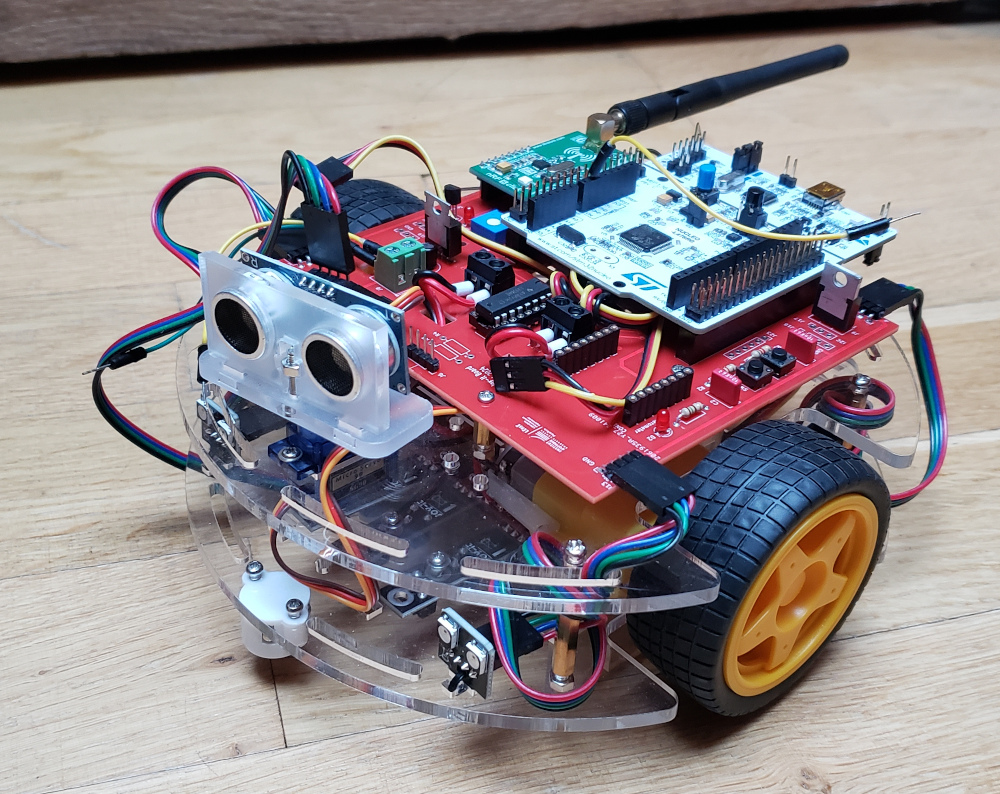
\includegraphics[width=0.4\textwidth]{images/robot_joycar.jpg}
\end{center}

\vfill

% Bottom of the page
%{\textbf{\large {Année universitaire} 2024-2025}}

\end{center}
\end{titlepage}

\newpage
\strut % empty page


%%%%%%%%%%%%%%%%%%%%%%%%%%%%%%%%%%%%%%%%%%%%%%%%
%%%%%%%%%%%%%    Intro
\newpage
\pagestyle{empty}

\begin{minipage}[c]{.25\linewidth}
	
\includegraphics[width=5cm]{images/Logo-LEnsE.png}
\end{minipage} \hfill
\begin{minipage}[c]{.4\linewidth}

\begin{center}
\vspace{0.3cm}
{\Large \textsc{Interfaçage Numérique}}

\medskip

6N-047-SCI \qquad \textbf{\Large Bloc Robot}

\end{center}
\end{minipage}\hfill

\vspace{0.5cm}

\noindent \rule{\linewidth}{1pt}

{\noindent\Large  \rule[-7pt]{0pt}{30pt} \textbf{Robotique et systèmes embarqués}}

\noindent \rule{\linewidth}{1pt}

\bigskip 

%%%%%%%%%%%%%%%%%%%%%%%%%%%%%%%%%%%%%%%%%%%%%%%%
%%%%%%%%%%%%%    A A V

{\large À l'issue des séances de TP concernant le \textbf{bloc de robotique} (4 séances), les étudiant$\cdot$es seront capables de ??? .}

\medskip

\textit{Ce sujet est disponible au format électronique sur le site du LEnsE - https://lense.institutoptique.fr/ dans la rubrique Année / Première Année / Interfaçage Numérique S6 / Bloc Robot.}

\noindent \rule{\linewidth}{1pt}

\medskip

Pour cela, ils$\cdot$elles seront capables de~:

\begin{itemize}
	\item ???
\end{itemize}

\noindent \rule{\linewidth}{1pt}


%%%%%%%%%%%%%%%%%%%%%%%%%%%%%%%%%%%%%%%%%%%%%%%%
%%%%%%%%%%%%%    Objectifs

\section{Objectifs du mini-projet}

L'objectif principal de ce mini-projet est de \textbf{développer le code embarqué d'une plateforme robotique} lui permettant : 

\begin{itemize}
	\item soit de se déplacer de manière autonome le long d'une ligne sans percuter d'obstacle.
	\item soit d'être piloter à distance par une télécommande et d'afficher des informations provenant de capteurs intégrés à la plateforme.
\end{itemize}

%%%%%%%%%%%%%%%%%%%%%%%%%%%%%%%%%%%%%%%%%%%%%%%%
%%%%%%%%%%%%%    Ressources

\section{Ressources}

Matériel : robot Joy-It car, télécommande, logiciel Arduino, carte Nucléo L476RG, capteurs, cartes de communication nRF24L01

\textit{Un descriptif des ressources de la plateforme robotique est disponible dans la suite de ce document.}

Tutoriaux Arduino

Codes d'exemple : Communication entre deux nRF24, affichage sur écran LCD...



%%%%%%%%%%%%%%%%%%%%%%%%%%%%%%%%%%%%%%%%%%%%%%%%
%%%%%%%%%%%%%    Déroulement

\section{Déroulement du bloc}

\textit{La liste des étapes à suivre pour la réalisation du programme embarqué de la plateforme robotique est donnée à titre indicatif. L'ordre et le choix des différentes étapes sont laissés à l'appréciation des différents binômes.}

\textit{Afin de faciliter la réutilisation des codes, il pourra être intéressant de définir des fonctions pour le pilotage des différents éléments.}

\subsection{Déplacements élémentaires}

Les deux premières séances sont communes sur la démarche de conception d'une application embarquée.


\subsubsection{Séance 1 - Prise en main de la maquette et premiers programmes Arduino}
\begin{description}
	\item[Etape 1 - 30 min] Piloter des sorties numériques - LED
	\item[Etape 2 - 30 min] Acquérir des données numériques - Bouton-poussoirs (interruptions)
	\item[Etape 3 - 60 min] Acquérir des données analogiques - Potentiomètres
	\item[Etape 4 - 30 min] Utiliser des sorties modulées en largeur d'impulsion (PWM) - LEDs
	\item[Etape 5 - 90 min] Piloter les deux moteurs du robot
\end{description}
	
	\bigskip

\subsubsection{Séance 2 - Capteurs et bibliothèques}
\begin{description}
	\item[Etape 6 - 60 min] Piloter les phares du robot à l'aide de la bibliothèque WS2812 (NeoPixel)
	\item[Etape 7 - 30 min] Acquérir des données du capteur de température analogique
	\item[Etape 8 - 60 min] Acquérir des données des capteurs de ligne
	\item[Etape 9 - 90 min] Acquérir des données de l'accéléromètre (I2C)
\end{description}



\subsection{Pilotage de haut niveau}

Les deux séances suivantes seront consacrées au pilotage du robot en fonction du cahier des charges choisi (suivi d'une ligne ou pilotage par une télécommande).

\subsubsection{Robot autonome / Suivi Ligne}

 \textit{Réalisable par un seul binôme}

\begin{description}
	\item[Etape A11 - 120 min] Définir et tester une première structure de code permettant de piloter les deux moteurs du robot en fonction de la détection des lignes
	\item[Etape A12 - 90 min] Acquérir les signaux du capteur ultrason
	\item[Etape A13 - 90 min] Piloter le servomoteur associé au capteur ultrason
	\item[Etape A14 - 180 min] Améliorer le programme de contrôle du robot
\end{description}
	

\subsubsection{Robot télécommandé}

 \textit{Réalisable par association de deux binômes, un binôme sur la télécommande (t) et un autre sur le robot (r)}


\begin{description}
	\item[Etape T11t - 60 min] Prendre en main la maquette de la télécommande
	\item[Etape T12t - 60 min] Acquérir les données provenant du joystick
	\item[Etape T11r - 120 min] Définir et tester une première structure de code permettant de piloter les deux moteurs du robot en fonction d'un ordre de direction
	\item[Etape T13 - 120 min] Utiliser la bibliothèque nRF24 pour mettre en place un échange de données entre la télécommande et le robot
	\item[Etape T14t - 60 min] Transmettre les données de direction depuis la télécommande vers le robot
	\item[Etape T14r - 60 min] Traduire les données de direction en ordre pour les moteurs du robot
	\item[Etape T15 - 180 min] Améliorer le programme de contrôle du robot (utilisation de l'écran LCD de la télécommande pour afficher la direction, les données de température, de l'accéléromètre...)		
\end{description}


\noindent \rule{\linewidth}{1pt}

\medskip

\textbf{\large Liste des autres ressources}
\begin{itemize}
	\item \textbf{Tutoriaux Arduino} :
	\begin{itemize}
		\item Projet Arduino et structure d'un code embarqué
		\item Entrées/Sorties Numériques
		\item Entrées Analogiques
		\item Sorties PWM
		\item Utilisation d'une bibliothèque
		\item Liaison série
		\item Liaison SPI / I2C
		\item Communication avec nRF24L01		
	\end{itemize}
	\item Pilotage d'un composant de puissance
	\item Mise en place d'un protocole d'échange de données
	
\end{itemize}


\newpage
\strut % empty page
%%%%%%%%%%%%%%%%%%%%%%%%%%%%%%%%%%%%%%%%%%%%%%%%
%%%%%%%%%%%%%    Séance 2 détaillée
\begin{minipage}[c]{.25\linewidth}
	
\includegraphics[width=4cm]{images/Logo-LEnsE.png}
\end{minipage} \hfill
\begin{minipage}[c]{.4\linewidth}

\begin{center}
\vspace{0.3cm}
{\Large \textsc{Interfaçage Numérique}}

\medskip

6N-047-SCI \qquad \textbf{\Large Bloc Robot}

\end{center}
\end{minipage}\hfill

\vspace{0.5cm}

\noindent \rule{\linewidth}{1pt}

{\noindent\Large \rule[-7pt]{0pt}{30pt} \textbf{Séance 2} / Capteurs et bibliothèques} 

\noindent \rule{\linewidth}{1pt}

\section{Etape 9 - Acquérir des données de l'accéléromètre (I2C)}

\begin{center} \textbf{\textit{Temps conseillé : 90 min}} \end{center}

Le composant que nous allons étudier est un \textbf{accéléromètre et magnétomètre} intégrés sur une même puce de silicium. Sa référence est \textbf{FXOS8700CQ}. Ce composant est intégré au module \textit{MikroE} \textbf{DOF6 - IMU Click}.

\subsection{Protocole I2C}

DESCRIPTION PROTOCOLE et CONNECTIQUES !

\bigskip

\textsc{Attention !} Les broches utilisées sur la carte Nucléo pour l'I2C ne sont pas celles par défaut. Il est indispensable de préciser les broches SDA et SCL à l'aide des méthodes suivantes :

\begin{lstlisting}
Wire.setSDA( PB9 );    
Wire.setSCL( PB8 ); 
\end{lstlisting}

\bigskip

\Manip Ouvrir le code \textsl{09\_accelero.ino} fourni. Compiler ce code et téléverser ce code dans la carte Nucléo.

Ce code contient les fonctions \textsl{test\_FXOS()} et \textsl{read\_i2c\_buffer()}, ainsi que des définitions des registres internes du composant.

\Manip 

\subsection{Configuration}


\subsection{Récupération des données}

\textit{These registers contain the X-axis, Y-axis, and Z-axis 14-bit left-justified sample data expressed as 2's complement numbers.} [NXP Doc p.52 of 113] 

\subsection{Traceur Série}

\begin{lstlisting}
  Serial.print(valeur1);
  Serial.print(",");
  Serial.print(valeur2);
  Serial.print(",");
  Serial.print(valeur3);
  Serial.print(",");
  Serial.print(valeur4);
  Serial.println();
\end{lstlisting}


\newpage
\strut % empty page
%%%%%%%%%%%%%%%%%%%%%%%%%%%%%%%%%%%%%%%%%%%%%%%%
%%%%%%%%%%%%%    Robot autonome
\begin{minipage}[c]{.25\linewidth}
	
\includegraphics[width=4cm]{images/Logo-LEnsE.png}
\end{minipage} \hfill
\begin{minipage}[c]{.4\linewidth}

\begin{center}
\vspace{0.3cm}
{\Large \textsc{Interfaçage Numérique}}

\medskip

6N-047-SCI \qquad \textbf{\Large Bloc Robot}

\end{center}
\end{minipage}\hfill

\vspace{0.5cm}

\noindent \rule{\linewidth}{1pt}

{\noindent\Large \rule[-7pt]{0pt}{30pt} \textbf{Pilotage} / Robot télécommandé} 

\noindent \rule{\linewidth}{1pt}


\section{Etape A13 - Piloter le servomoteur associé au capteur ultrason}

\textit{Temps conseillé : 90 min}

\subsubsection{Utilisation de la sortie modulée PB7}
	
\begin{lstlisting}
LL_GPIO_SetAFPin_0_7(GPIOB,  GPIO_PIN_7,  GPIO_AF1_TIM2);
\end{lstlisting}

\newpage
\strut % empty page
%%%%%%%%%%%%%%%%%%%%%%%%%%%%%%%%%%%%%%%%%%%%%%%%
%%%%%%%%%%%%%    Robot télécommandé
\begin{minipage}[c]{.25\linewidth}
	
\includegraphics[width=4cm]{images/Logo-LEnsE.png}
\end{minipage} \hfill
\begin{minipage}[c]{.4\linewidth}

\begin{center}
\vspace{0.3cm}
{\Large \textsc{Interfaçage Numérique}}

\medskip

6N-047-SCI \qquad \textbf{\Large Bloc Robot}

\end{center}
\end{minipage}\hfill

\vspace{0.5cm}

\noindent \rule{\linewidth}{1pt}

{\noindent\Large \rule[-7pt]{0pt}{30pt} \textbf{Pilotage} / Robot télécommandé} 

\noindent \rule{\linewidth}{1pt}

\section{Etape T13 - Communication avec des modules nRF24L01}

Installation de la bibliothèque \textbf{RF24} sur \textit{Arduino}.

\subsection{Protocole SPI}


\subsubsection{Changer les broches par défaut pour la liaison SPI}

Ces lignes doivent être exécutées AVANT de démarrer logiciellement le module nRF24 (avant la ligne \textsl{radio.begin()} ).

\begin{lstlisting}
SPI.setMISO(SPI_MISO);
SPI.setMOSI(SPI_MOSI);
SPI.setSCLK(SPI_SCK);
\end{lstlisting}


Côté robot : 

\begin{lstlisting}
#define   NRF_CE    PD2
#define   NRF_CSN   PA14
#define   NRF_INT   PA15
#define   SPI_SCK   PC10
#define   SPI_MISO  PC11
#define   SPI_MOSI  PC12
\end{lstlisting}


Côté télécommande : 

\begin{lstlisting}
#define   NRF_CE    PA15
#define   NRF_CSN   PB7
#define   NRF_INT   PA14
#define   SPI_SCK   PA5
#define   SPI_MISO  PA6
#define   SPI_MOSI  PA7
\end{lstlisting}

\newpage
\strut % empty page

%%%%%%%%%%%%%%%%%%%%%%%%%%%%%%%%%%%%%%%%%%%%%%%%
%%%%%%%%%%%%%    Présentation de la maquette
\newpage
\begin{minipage}[c]{.25\linewidth}
	
\includegraphics[width=4cm]{images/Logo-LEnsE.png}
\end{minipage} \hfill
\begin{minipage}[c]{.4\linewidth}

\begin{center}
\vspace{0.3cm}
{\Large \textsc{Interfaçage Numérique}}

\medskip

6N-047-SCI \qquad \textbf{\Large Bloc Robot}

\end{center}
\end{minipage}\hfill

\vspace{0.5cm}

\noindent \rule{\linewidth}{1pt}

{\noindent\Large \rule[-7pt]{0pt}{30pt} \textbf{Robot Joy-It Car} / Présentation du matériel}

\noindent \rule{\linewidth}{1pt}

\bigskip

{\LARGE La tension maximale admissible par les moteurs est de $7\operatorname{V}$ !}

\bigskip

\noindent \rule{\linewidth}{1pt}


%%%%%%%%%%%%%%%%%%%%%%%%%%%%%%%%%%%%%%%%%%%%%%%%
%%% RESSOURCES COMPLEMENTAIRES		

\newpage
% Ressources
\begin{center}
	\begin{minipage}{2.5cm}
	\begin{center}
		
\includegraphics[width=5cm]{images/Logo-LEnsE.png}
	\end{center}
\end{minipage}\hfill
\begin{minipage}{10cm}
	\begin{center}
	\textbf{Institut d'Optique Graduate School }\\[0.1cm]
    \textbf{Interfaçage Numérique}


	\end{center}
\end{minipage}\hfill


\vspace{2cm}


{\Large \bfseries \textsc{Interfaçage Numérique}} \\[0.5cm]
{\large \bfseries Travaux Pratiques} \\[0.2cm]
Semestre 6

\vspace{1cm}

% Title
\rule{\linewidth}{0.4mm} \\[0.4cm]
{ \Large \bfseries\color{violet_iogs} Ressources \\[0.4cm] }
\rule{\linewidth}{0.4mm} \\[1cm]
{\large Bloc Robot}

\end{center}

\vspace{3cm}

\textbf{\large Liste des ressources}
\begin{itemize}
	\item \hyperref[doc:robot_schematic]{Schéma de la carte du robot Joy-It Car}
	\item \hyperref[doc:robot_pcb]{PCB de la carte du robot Joy-It Car}
\end{itemize}

\vfill

\newpage
\strut % empty page
% Ressources
\titleformat{\section}
  {\null}{}{0pt}{}


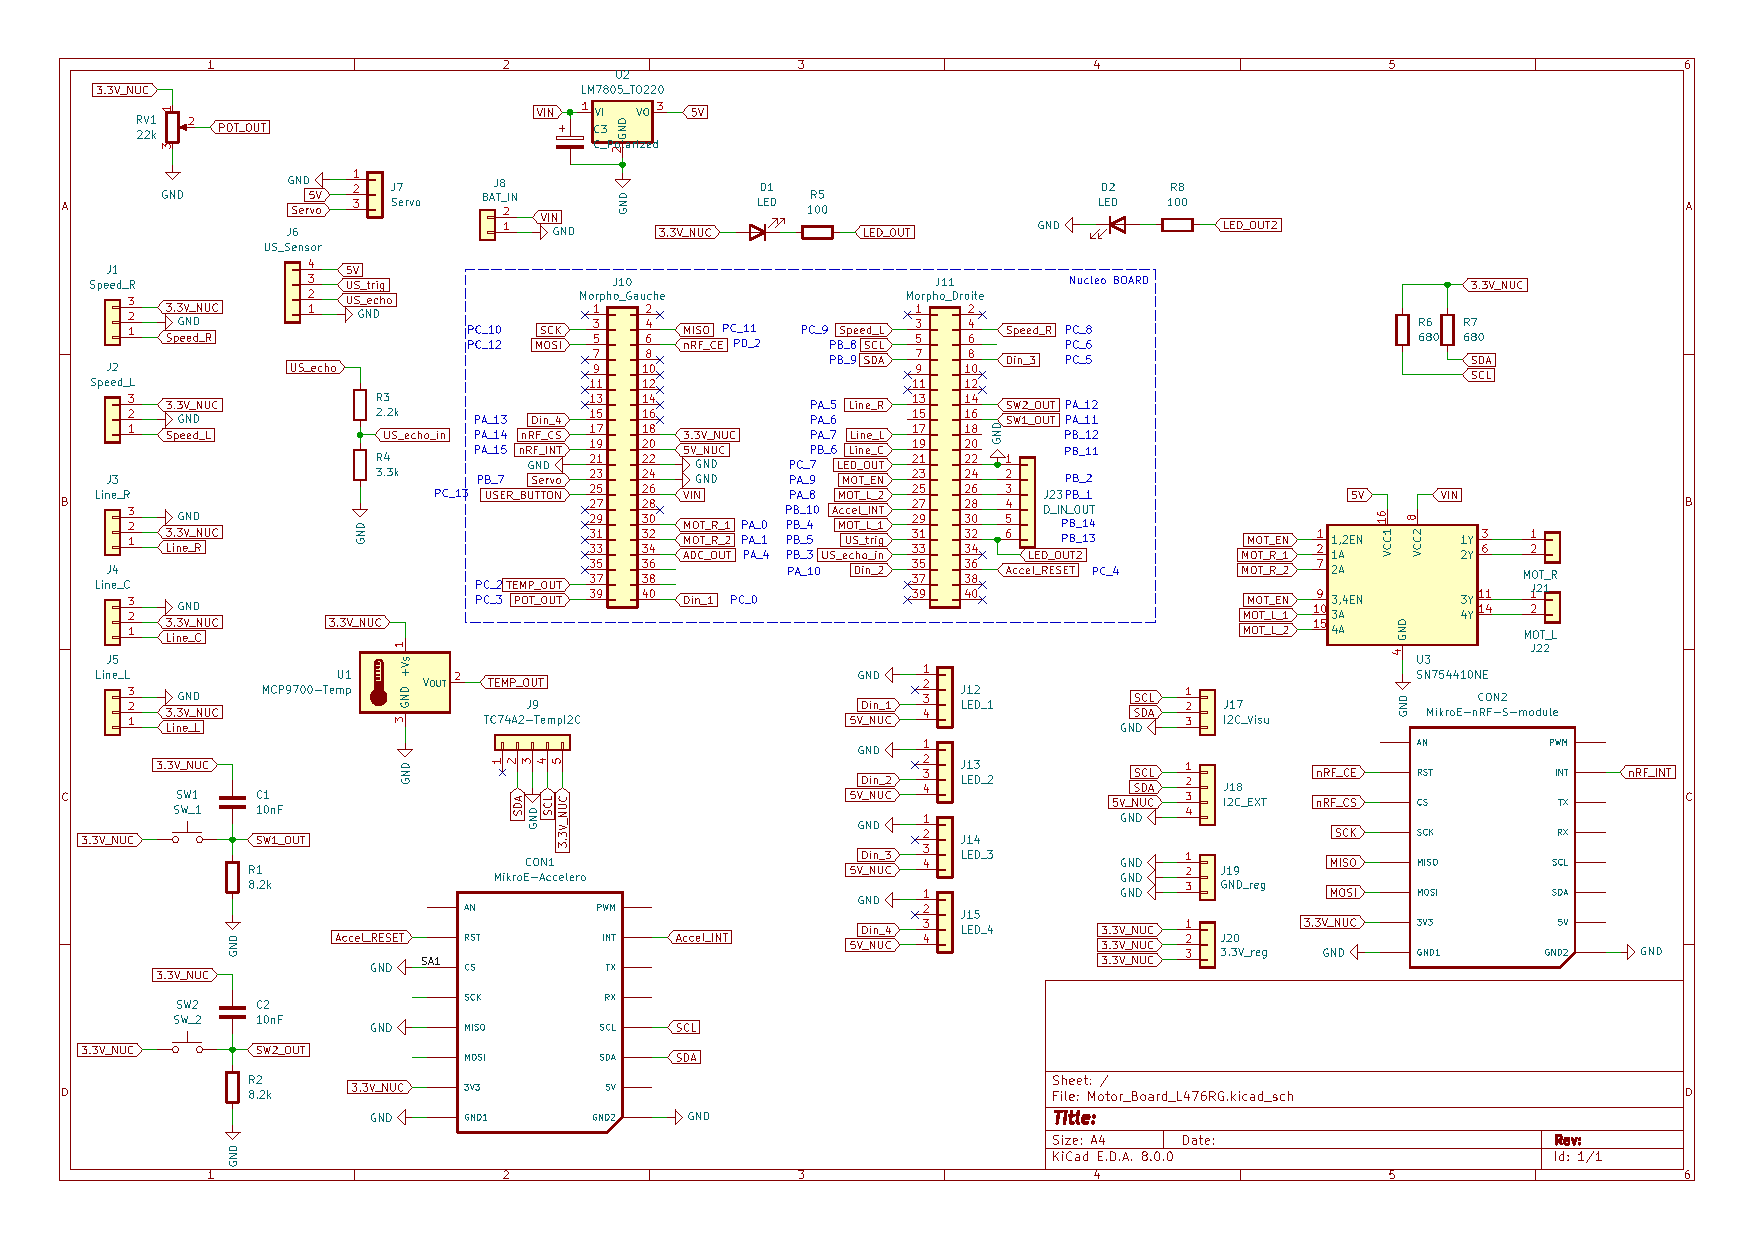
\includepdf[pages=1, landscape=true, pagecommand={\section{\texorpdfstring{\hspace{-1em}}{Schéma Robot}}}\label{doc:robot_schematic}]{ressources/Motor_Board_L476RG_sch.pdf}


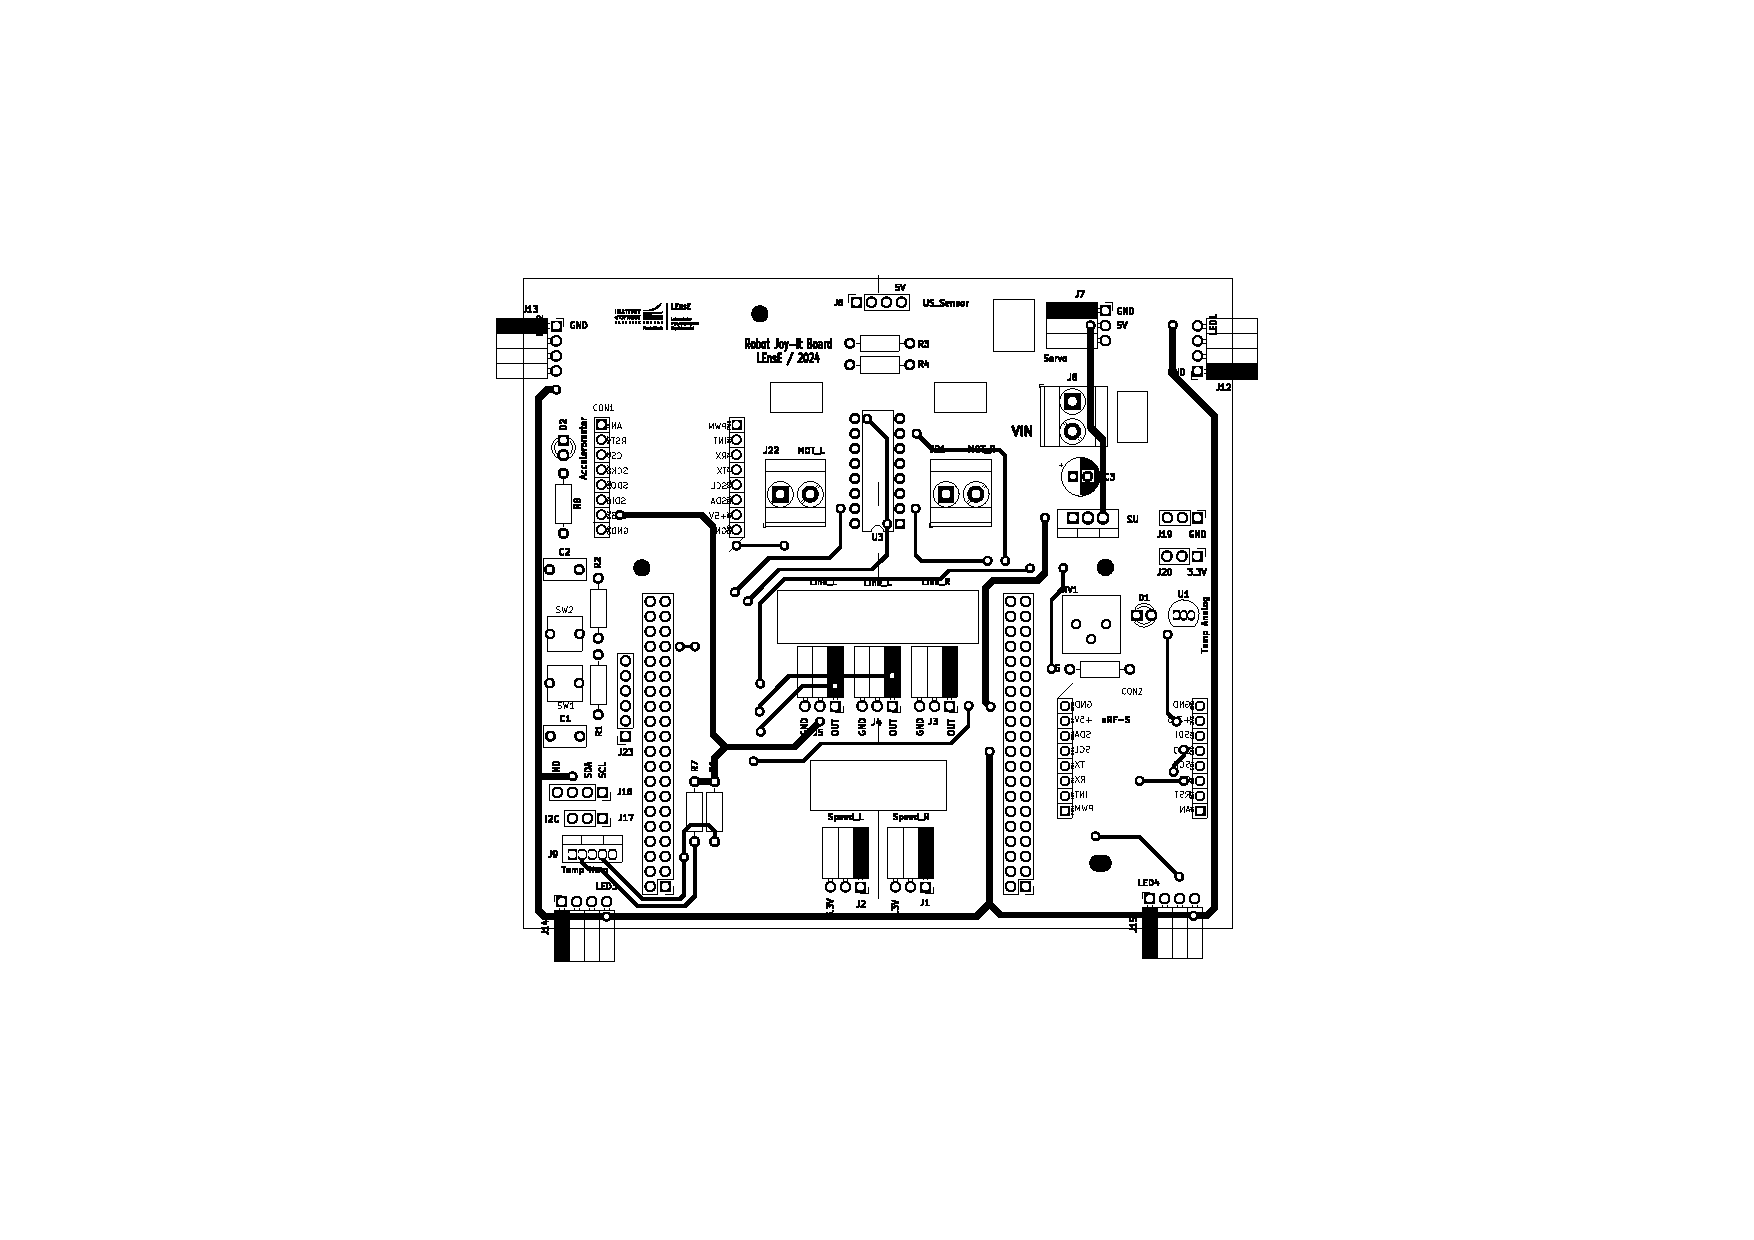
\includepdf[pages=1, landscape=true, pagecommand={\section{\texorpdfstring{\hspace{-1em}}{PCB Robot}}}\label{doc:robot_pcb}]{ressources/Motor_Board_L476RG_pcb.pdf}


\end{document}


